% !TEX root = memoire.tex
\chapter{G\'en\'eration exaustive}\label{chapitre-generation}

\vspace{-1em}
Dans ce chapitre nous présentons un algorithme de génération exhaustive basé sur le parcours du bord extérieur d'un polyomino.

Si nous connaissons le polyomino à l'avance, il existe un parcours canonique de son bord de longueur minimale. Pour l'obtenir nous avons besoin de deux choses: un point de départ canonique sur le bord et une orientation du parcours. Ensuite, à partir de ce point de départ, on se déplace de manière à longer le bord du polyomino. 

Nous présentons la classe des polyominos ainsi énumérés ainsi que leur représentation à l'aide de pierres de \Go dans la section $1$. Dans la section $2$, nous décrirons un jeu basé sur le \Go dont une partie terminée représente un polyomino délimité par un nombre donné de pierres noires. Nous terminerons le chapitre avec la section $3$, où nous présentons l'algorithme de génération exhaustive ainsi qu'une spécialisation pour les polyominos avec différents types de trou.


\vspace{-1em}
\section{Les gominos}

%On considère les chemins codés par les lettres de l'alphabet $\mathcal{A}=\{0,1,2,3,4,5,6,7\}$. Un sous-ensemble $S\subseteq\Z^2$ est \emph{$4$-connexe} (resp. \emph{$8$-connexe}) si toute paire de points est reliée par un $4$-chemin (resp. $8$-chemin). Un \emph{polyomino} $P$ est un ensemble fini $4$-connexe, habituellement représenté à l'aide de carrés unités dans le plan $\Z^2$.

\vspace{-0.5em}
On considère $\Z^2$ comme une planche de \Go infinie et on y représente le contour extérieur $P^+$ d'un polyomino $P$ à l'aide de pierres noires, et le contour intérieur $P^-$ à l'aide de pierres blanches tel qu'illustré à la figure \ref{fig:polyomino-et-gomino}. 

\begin{definition}\label{def:gomino}
Un \emph{gomino} est une paire $G=\left( P^+,P^- \right)$ d'ensembles dans $\Z^2$ pour lesquels il existe un polyomino $P$ tel que $P^+$ est son contour extérieur et $P^-$ est son contour intérieur.
\end{definition}

\begin{figure}[h]
\centering
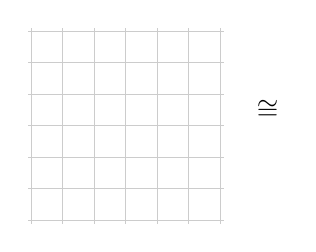
\begin{tikzpicture}[scale=.4, tile/.style={draw, blue!60!black, fill=blue!10, rectangle, inner sep=0.2cm}]
\draw[color=black!20] (-2.1,-1.1) grid (4.1,5.1);
\squarepath{(-1,2)}{66000222446602};
\node[draw=none,fill=none] at (5.5,2.5) {$\cong$}; 
\end{tikzpicture} 
\hspace{.5cm}
\begin{tikzpicture}[scale=.4, every node/.style={scale=.4, minimum size=1cm}, node distance=1cm] 
\goban{6}{6} 
\whitestonepath{(1,3)}{66000222446};
\blackstonepath{(0,3)}{667000122234455};
\end{tikzpicture}

\caption{Un polyomino simplement $4$-connexe et son gomino.}\label{fig:polyomino-et-gomino}
\end{figure}

L'analogie avec le \Go, autre que le fait d'utiliser des pierres noires et blanches, réside dans le fait que selon la terminologie du \Go, un polyomino simplement $4$-connexe $P$ avec son contour $P^+$ est le \emph{territoire noir}, et $P^+$ délimite ce territoire de façon minimale. L'algorithme décrit plus loin génère chaque gomino avec $n$ pierres noires, donc chaque polyomino de périmètre de site $n$, en plaçant tour à tour des pierres noires et blanches, comme le feraient deux joueurs de \Go.


\section{Un jeu bien solitaire}

Le jeu de \textit{Gomino} est d'une certaine façon une version simplifiée du jeu de \Go. D'une position initiale, deux joueurs $\B$ et $\W$ jouent sur une planche de jeu $\N \times \Z$ en laissant des pierres sur chaque point de la grille visité et libre jusque là. $\B$ a $n$ pierres noires en main et tente d'encercler un territoire en revenant à sa position d'origine, tandis que $\W$ essaie de l'en empêcher en plaçant des pierres blanches.

On décrit la séquence des positions successives de chacun des joueurs à l'aide deux fonctions
\[\B, \W: \N \to \N\times\Z,\]
dont on fixe les points de départ
\begin{equation}\label{CI}
\B(0)= (0,0)  \quad;\quad
\W(0) = (1,0).
\end{equation}

La notion suivante est utile pour décrire les $4$-trous.

\begin{definition}
Un \emph{motif en X} est un alignement de pierres $2\times2$ tel que l'une de ses diagonales est noire, et l'autre blanche.
\end{definition}

\begin{figure}[h!]
\centering

\begin{subfigure}[b]{.4\textwidth}
\centering
\begin{tikzpicture}[every node/.style={minimum size=1cm}, node distance=1cm]
\gobanc{2}{2}
\wm{(0,0)} \wm{(1,1)}
\bm{(0,1)} \bm{(1,0)}
\end{tikzpicture}
\end{subfigure}
\begin{subfigure}[b]{.4\textwidth}
\centering
\begin{tikzpicture}[every node/.style={minimum size=1cm}, node distance=1cm]
\gobanc{2}{2}
\bm{(0,0)} \bm{(1,1)}
\wm{(0,1)} \wm{(1,0)}
\end{tikzpicture}
\end{subfigure}
\caption{Motifs en X}
\end{figure}

\subsection{Position de départ et zones interdites}

Afin de rendre chaque parcours unique et éviter la répétition de polyominos par translation, on choisit une cellule du polyomino $P$, appellée la \emph{racine} de $P$. L'une des manières d'obtenir canoniquement une telle cellule est d'utiliser la factorisation standard tel qu'illustré  à la figure \ref{fig:NSEW} et de choisir la cellule ayant comme sommet le point $W$.

\begin{figure}
\centering
\shorthandoff{:}
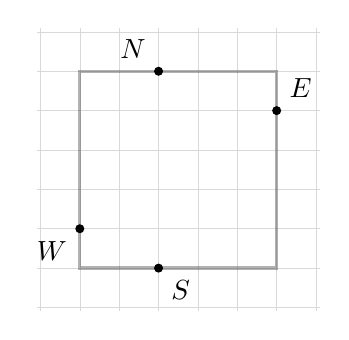
\begin{tikzpicture}[polyomino/.style={black, fill=red, fill opacity=0.3, very thick}, >=latex, scale=0.5]
	\squarepath{(1,2)}{06200244202060};
	\draw[help lines, opacity=0.3] (-0.1,-0.1) grid (7.1, 7.1);
	\draw[very thick, opacity=0.3] (1,1) rectangle (6,6);
	\node[circle, draw, fill, inner sep=1, label=below left:{$W$}] at (1,2) {};
	\node[circle, draw, fill, inner sep=1, label=below right:{$S$}] at (3,1) {};
	\node[circle, draw, fill, inner sep=1, label=above right:{$E$}] at (6,5) {};
	\node[circle, draw, fill, inner sep=1, label=above left:{$N$}] at (3,6) {};
\end{tikzpicture}
\caption{Factorisation NSEW du contour}\label{fig:NSEW}
\end{figure}

Pour s'assurer de respecter les contraintes imposées par le choix de la racine, on interdit à $\B$ de jouer sous sa position initiale en colonne $0$ et à $\W$ de jouer sur la colonne $0$. Ces positions sont appelées \emph{zones interdites}.

\begin{figure}[H]
\centering
\begin{tikzpicture}
\goban{5}{5}
\node[opacity=0.25] at (0,0) {\blackstone};
\node at (0,0) [forbidden sign,line width=0.3ex,draw=red]{};
\node[opacity=0.25] at (0,1) {\blackstone};
\node at (0,1) [forbidden sign,line width=0.3ex,draw=red]{};
\node at (0,2) {\blackstone};
\node at (1,2) {\whitestone};
\node[opacity=0.25] at (0,3) {\whitestone};
\node at (0,3) [forbidden sign,line width=0.3ex,draw=red]{};
\node[opacity=0.25] at (0,4) {\whitestone};
\node at (0,4) [forbidden sign,line width=0.3ex,draw=red]{};
\end{tikzpicture}

\caption{Position de départ et zones interdites}
\end{figure}

\subsection{Règles de déplacement}
Le joueur $\B$ commence, et les joueurs jouent à tour de de rôle (figure \ref{figure:anatomie-coup}).

La liste des coups possibles est illustrée à la figure \ref{fig:regles-de-deplacement}. La pierre noire marquée en vert indique la position de $\B$, tandis que la pierre blanche marquée en vert qui y est $4$-connexe indique celle de $\W$. Les règles sont les suivantes:

\begin{figure}
\centering
\begin{subfigure}[b]{.3\textwidth}
\centering
\begin{tikzpicture}
\gobanc{3}{3}
\wm{(1,0)}
\bm{(1,1)}
\end{tikzpicture}
\caption{Position initiale}
\end{subfigure}
\begin{subfigure}[b]{.3\textwidth}
\centering
\begin{tikzpicture}
\gobanc{3}{3}
\wm{(1,0)}
\bm{(1,1)}
\bm{(2,2)}
\markstone{2}{2}
\end{tikzpicture}
\caption{Coup de $\B$}
\end{subfigure}
\begin{subfigure}[b]{.3\textwidth}
\centering
\begin{tikzpicture}
\gobanc{3}{3}
\whitestonepath{(1,0)}{4220}
\bm{(1,1)}
\bm{(2,2)}
\markstone[green!90!black]{0}{0}
\markstone[green!90!black]{0}{1}
\markstone[green!90!black]{0}{2}
\markstone[green!90!black]{1}{2}
\end{tikzpicture}
\caption{Réplique de $\W$}
\end{subfigure}
\caption{L'anatomie d'un coup}\label{figure:anatomie-coup}
\end{figure}




\begin{figure}[h!]
\begin{center}
\tikzstyle{level 1}=[sibling angle=(360/8), level distance=22mm]
\tikzstyle{level 2}=[sibling angle=(360/8), level distance=28mm]
\tikzstyle{every node}=[]
\tikzstyle{edge from parent}=[->, draw]
\begin{tikzpicture}[auto, >=latex, grow cyclic, clockwise from=90]
\node (ref) {\kifuc[scale=.2]{3}{\wm{(1,0)}\bm{(1,1)}}}
child {node[scale=.3] (a)  {\begin{tikzpicture}[every node/.style={minimum size=1cm}, node distance=1cm]
	\gobanc{3}{3};
	\wm{(1,0)}
	\bm{(1,1)}
	\bm{(1,2)}
	\markstone{1}{2};
\end{tikzpicture}}
  child[clockwise from=(90)] {node[scale=.7]{\begin{tikzpicture}[every node/.style={minimum size=1cm}, node distance=1cm]
	\goban{3}{3}
	\wm{(1,0)}
	\bm{(1,1)}
	\bm{(1,2)}
	\wm{(0,0)}
	\wm{(0,1)}
	\wm{(0,2)}	
	\markstone{0}{0}
	\markstone{0}{1}
	\markstone{0}{2}
\end{tikzpicture}
} edge from parent}
edge from parent}
child {node[scale=.3] (b) {\begin{tikzpicture}[every node/.style={minimum size=1cm}, node distance=1cm]
	\gobanc{3}{3};
	\wm{(1,0)}
	\bm{(1,1)}
	\bm{(2,2)}
	\markstone{2}{2};
\end{tikzpicture}}
  child[clockwise from=(45)] {node[scale=.7]{\begin{tikzpicture}[every node/.style={minimum size=1cm}, node distance=1cm]
	\goban{3}{3}
	\wm{(1,0)}
	\bm{(1,1)}
	\bm{(2,2)}
	\wm{(0,0)}
	\wm{(0,1)}
	\wm{(0,2)}	
	\wm{(1,2)}
	\markstone{0}{0}
	\markstone{0}{1}
	\markstone{0}{2}
	\markstone{1}{2}
\end{tikzpicture}
} edge from parent}
edge from parent[swap]}
child {node[scale=.3] (c) {\begin{tikzpicture}[every node/.style={minimum size=1cm}, node distance=1cm]
	\gobanc{3}{3};
	\wm{(1,0)}
	\bm{(1,1)}
	\bm{(2,1)}
	\markstone{2}{1};
\end{tikzpicture}}
  [clockwise from=0]
  child {node[scale=.7]{\begin{tikzpicture}[every node/.style={minimum size=1cm}, node distance=1cm]
	\goban{3}{3}
	\wm{(1,0)}
	\bm{(1,1)}
	\bm{(2,1)}
	\wm{(0,0)}
	\wm{(0,1)}
	\wm{(0,2)}	
	\wm{(1,2)}
	\wm{(2,2)}
	\markstone{0}{0}
	\markstone{0}{1}
	\markstone{0}{2}
	\markstone{1}{2}
	\markstone{2}{2}
\end{tikzpicture}
} edge from parent}
edge from parent[swap]}
child {node[scale=.3] (d) {n\begin{tikzpicture}[every node/.style={minimum size=1cm}, node distance=1cm]
	\gobanc{3}{3};
	\wm{(1,0)}
	\bm{(1,1)}
	\bm{(2,0)}
	\markstone{2}{0};
\end{tikzpicture}}
  [clockwise from=-45]
  child[sibling angle=45] {node[scale=.7]{\begin{tikzpicture}[every node/.style={minimum size=1cm}, node distance=1cm]
	\goban{3}{3}
	\wm{(1,0)}
	\bm{(1,1)}
	\bm{(2,0)}
	\wm{(0,0)}
	\wm{(0,1)}
	\wm{(0,2)}	
	\wm{(1,2)}
	\wm{(2,2)}
	\wm{(2,1)}
	\markstone{0}{0}
	\markstone{0}{1}
	\markstone{0}{2}
	\markstone{1}{2}
	\markstone{2}{2}
	\markstone{2}{1}
\end{tikzpicture}
} edge from parent}
 edge from parent[swap]}
child[missing] {}
child {node[scale=.3] (B) {\begin{tikzpicture}[every node/.style={minimum size=1cm}, node distance=1cm]
	\gobanc{3}{3};
	\wm{(1,0)}
	\bm{(1,1)}
	\bm{(0,0)}
	\markstone{0}{0};
\end{tikzpicture}}
  [clockwise from=-180+45]
  child {node[scale=.7]{\begin{tikzpicture}[every node/.style={minimum size=1cm}, node distance=1cm]
	\gobanc{3}{3};
	\wm{(1,0)}
	\bm{(1,1)}
	\bm{(0,0)}
\end{tikzpicture}} edge from parent}
 edge from parent}
child {node[scale=.3] (C) {\begin{tikzpicture}[every node/.style={minimum size=1cm}, node distance=1cm]
	\gobanc{3}{3};
	\wm{(1,0)}
	\bm{(1,1)}
	\bm{(0,1)}
	\markstone{0}{1};
\end{tikzpicture}}
  [clockwise from=(180)]
  child {node[scale=.7]{\begin{tikzpicture}[every node/.style={minimum size=1cm}, node distance=1cm]
	\gobanc{3}{3};
	\wm{(1,0)}
	\bm{(1,1)}
	\bm{(0,1)}
	\wm{(0,0)}
	\markstone{0}{0};
\end{tikzpicture}} edge from parent}
edge from parent}
child {node[scale=.3] (D) {\begin{tikzpicture}[every node/.style={minimum size=1cm}, node distance=1cm]
	\gobanc{3}{3};
	\wm{(1,0)}
	\bm{(1,1)}
	\bm{(0,2)}
	\markstone{0}{2};
\end{tikzpicture}}
  [clockwise from=(180-45)]
  child[sibling angle=45] {node[scale=.7]{\begin{tikzpicture}[every node/.style={minimum size=1cm}, node distance=1cm]
	\gobanc{3}{3};
	\wm{(1,0)}
	\bm{(1,1)}
	\bm{(0,2)}
	\wm{(0,0)}
	\wm{(0,1)}
	\markstone{0}{0};
	\markstone{0}{1};
\end{tikzpicture}} edge from parent}
edge from parent}
;
\end{tikzpicture}
\end{center}
\caption{Coups permis (à rotation près)}
\label{fig:regles-de-deplacement}
\end{figure}

\begin{itemize}
\item[$\B$:] ce joueur se déplace exactement d'un pas dans son $8$-voisinage excluant la zone interdite et les positions déjà occupées par des pierres blanches. On remarque que seuls les déplacements vers des intersections libres augmentent le nombre de pierres noires en jeu. De plus, $\B$ doit jouer son premier coup en direction \ocr{7}. Cette contrainte force $\B$ à parcourir le bord du polyomino en sens anti-horaire.

\item[$\W$:] ce joueur doit terminer son coup dans le $4$-voisinage de $\B$ en un nombre minimal de pas, de $0$ à $6$ selon le coup de $\B$. Il peut le faire en effectuant autant de pas qu'il le faut sur les intersections vides ou sur les pierres blanches dans le $8$-voisinage de la position précédente de $\B$ tout en respectant les conditions suivantes:

\begin{enumerate}
\item \emph{Règle de la main droite.} À la fin de chaque tour, $\W$ doit être situé à gauche de la flèche décrivant le dernier coup de $\B$.

Cette règle force $\W$ à rester à l'intérieur du polyomino dont le bord extérieur est construit par $\B$.

\item \emph{Règle des trous.} $\W$ ne peut en aucun cas former de motif en X.

La règle des trous évite de créer des polyominos contenant des $8$-trous et ainsi assure que tous les polyominos générés par l'algorithme seront simplement $4$-connexe. Cette contrainte sera relâchée plus tard lorsque nous adapterons l'algorithme pour obtenir les polyominos contenant les différents types de trous.
\end{enumerate}
\end{itemize}

\vspace{-0.5em}
Pour comprendre l'ajout de plusieurs pierres blanches en un seul coup, on doit se rappeler que par définition, $\B$ encercle $\W$ avec un minimum de pierres. Chaque coup de $\B$ nous révèle donc un peu plus d'information sur $\W$. En particulier, si $\W$ peut jouer une pierre alors on sait que cet emplacement fait bien partie de $\W$ puisque dans le cas contraire $\B$ aurait tout simplement joué là au tour précédent et ainsi bloqué $\W$.

On remarque aussi que la séquence qui mène à l'ajout de 6 pierres est interdite par la règle des trous et donc n'est pas un coup valide pour $\W$. Elle sera par contre utilisée plus loin pour générer les polyominos simplement $8$-connexes.

Finalement, la restriction de $\W$ sur la colonne $0$ garanti que si $\B$ joue sur la colonne $-1$ on a une victoire de $\W$. Puisqu'on cherche à énumérer les victoires de $\B$, on évitera d'y jouer.

\vspace{-0.5em}
\subsection{Fin de partie}

\vspace{-0.5em}
On dit que \emph{$\B$ gagne} s'il parvient à revenir à sa position d'origine. Dans ce cas, les chemins parcourus par $\B$ et $\W$ décrivent respectivement le contour extérieur et intérieur d'un unique polyomino $P$.

Si à n'importe quelle étape, $\W$ est incapable de rejoindre le $4$-voisinage de $\B$ en utilisant un coup permis, alors $\W$ gagne. De plus, quand aucune séquence de coups ne mène à une victoire de $\B$, alors $\W$ gagne. En conséquence, il y a bijection entre les polyominos et les parties de Gomino gagnées par $\B$.

\begin{theorem}\label{thm:G=P}
Tout polyomino simplement $4$-connexe $P$ est décrit par une unique partie de gomino $G$ gagnée par $\B$.
\end{theorem}

\begin{proof}
Soit $P$ un polyomino simplement $4$-connexe, $P^+$ et $P^-$ ses contours extérieurs et intérieurs. On construit, par induction, une partie de Gomino qui décrit $P$ et on montre que cette partie est unique.

On débute avec $\B(0)$ et $\W(0)$ tel que décrit par l'équation \eqref{CI}, et on identifie $\W(0)$ à la racine de $P$. Puisque le premier coup de $\B$ doit absolument être $0$, on a que $\B(1)=(1,-1)$, qui est un point de $P^+$, et $\W(1)=(1,0)$, qui est un point de $P^-$.

Supposons maintenant que $\B$ a déjà joué $n$ coups tels que chaque pierre noire placée jusqu'à maintenant est dans $P^+$ et chaque pierre blanche est dans $P^-$. Soit $\vec{b}_n$ la flèche de $\B(n-1)$ vers $\B(n)$. À l'étape $n$, nous sommes, à rotation près, dans la situation illustrée à la figure \ref{fig:ordre}. Certaines intersections peuvent contenir des pierres. On numérote les intersections en commençant à $0$ à partir de $\W(n)$.

\begin{figure}[h!]
\centering
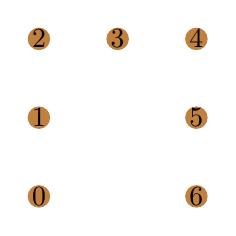
\begin{tikzpicture}[every node/.style={scale=1}, marker/.style={fill=brown, inner sep=0, circle}]
	\gobanc{3}{3}
	\wm{(1,0)}
	\bm{(1,1)}
	\markstone[green!90!black]{1}{0}
	\markstone{1}{1}
\node[marker] at (0,0) {\circled{0}};
\node[marker] at (0,1) {\circled{1}};
\node[marker] at (0,2) {\circled{2}};
\node[marker] at (1,2) {\circled{3}};
\node[marker] at (2,2) {\circled{4}};
\node[marker] at (2,1) {\circled{5}};
\node[marker] at (2,0) {\circled{6}};
\end{tikzpicture}
\caption{Ordre du $8$-voisinage}
\label{fig:ordre}
\end{figure}

On remarque qu'en numérotant le voisinage de $\B(n)$ en sens horaire en commençant à $\W(n)$, le point $\B(n+1)$ est le premier point de $P^+$ rencontré. En effet, lorsque $\B$ place une pierre en $i$, $\W$ réplique en plaçant ses pierres en $1,2,\dots, i-1$, ce qu'il peut toujours faire puisque ces positions sont libres et dans le $8$-voisinage de $\B(n)$. S'il existait une position $j<i$ contenant déjà une pierre noire, alors $\W$ serait incapable de se connecter à la nouvelle position de $\B$ et serait victorieux donc la partie ne représenterait pas $P$. De même, s'il existe une position $j<i$ qui contiendra éventuellement une pierre noire, $\B$ doit obligatoirement jouer sur ce point de $P^+$, sinon $\W$ y placera une pierre blanche et notre gomino ne représentera plus $P$.
\end{proof}

\paragraph*{Remarque:} Une conséquence directe du théorème 1 est que la séquence des coups joués par $\B$ lors d'une victoire, codée par un mot sur $\mathcal{A}$, est suffisante pour décrire un polyomino unique. Par exemple, le polyomino illustré à la figure \ref{fig:polyomino-et-gomino} est encodé par le mot $w=\ocr{700012223445566}$.



\section{L'algorithme de génération}

\vspace{-0.5em}
Nous utilisons maintenant la bijection entre les parties de Gomino et les polyominos pour décrire notre principal algorithme qui permet la génération exhaustive des polyominos simplement $4$-connexes. Nous parlerons simplement de \emph{l'algorithme des gominos}. Lorsque nous faisons référence à une partie de gomino, celle-ci peut être inachevée.

\vspace{-0.5em}
\paragraph{\bf L'algorithme des gominos.} {\it L'algorithme accepte en entrée une partie de gomino de $n$ coups et retourne en sortie la liste des parties de $(n+1)$ coups possibles à partir de ce point.

\vspace{-0.5em}
\begin{enumerate}
\item \emph {Construire la liste des coups valides}

D'abord le coup de $\B$: toute intersection vide ou contenant une pierre noire dans le $8$-voisinage de la position actuelle de $\B$ est un coup valide. $\W$ répond immédiatement et comme il est montré à la figure \ref{fig:regles-de-deplacement}, a un seul coup possible. Si $\W$ est incapable de jouer, rejeter ce coup immédiatement. Sinon, l'ajouter à la liste.

\item \emph{Créer de nouvelles parties}

Pour chaque coup valide, créer une copie de la partie actuelle, y jouer ce coup et ajouter la partie à l'ensemble des nouvelles parties. Pour chaque partie de $n$ coups, l'algorithme peut créer jusqu'à sept nouvelles parties de $(n+1)$ coups. La partie reçue en paramètre par l'algorithme n'est plus utilisée par la suite et peut être effacée à ce moment.

\item \emph{Comptabiliser les victoires}

Les conditions de victoires sont vérifiées sur chaque nouvelle partie. Les victoires de $\W$ sont rejetées et les victoires de $\B$ sont conservées (ce sont nos polyominos). Puis les autres parties sont ajoutées à l'ensemble des parties en cours.

\item \emph{Appliquer récursivement}

On applique ensuite l'algorithme récursivement sur chacune des parties en cours, jusqu'à ce que cet ensemble soit vide. Puisque chaque partie est indépendante des autres, cette étape peut être traitée en parallèle.
\end{enumerate}

}


\vspace{-0.5em}
\subsection{$4$-trous} \label{subsection:4-trous}

\vspace{-0.5em}
Nous présentons maintenant une extension de l'algorithme de base qui permet de générer les polyominos simplement $8$-connexes en retirant la règle des trous. Le coup blanc \ocr{422006} devient alors valide et décrit un trou d'aire $1$.

Notons que la preuve du théorème \ref{thm:G=P} ne fait aucune mention de $4$-trous. Conséquemment, le théorème reste vrai pour les polyominos simplement $8$-connexes incluant des motifs en X. Bien que ces motifs soient permis pour les polyominos simplement $8$-connexes, nous pouvons les utiliser pour compter les $4$-trous.

\begin{proposition}
Si un gomino $G$ décrit un polyomino simplement $8$-connexe $P$, alors il y a autant de motif en X dans $G$ qu'il y a de $4$-trous dans $P$.
\end{proposition}

\vspace{-0.5em}
\begin{proof}
Procédons par induction sur le nombre de $4$-trous dans un polyomino $P$.
Considérons tout d'abord le cas d'un seul $4$-trou. Il y a au moins un motif en X, puisque c'est le seul motif qui bloque tout $4$-chemin de l'intérieur vers l'extérieur du trou tout en permettant l'existence de $8$-chemin. S'il y avait un $4$-chemin de l'intérieur vers l'extérieur, alors ce ne serait pas un trou. D'un autre coté, si on suppose l'existence de deux motifs en X, alors il existe deux $8$-chemins reliant l'intérieur du trou à l'extérieur. Prenons deux points, par exemple $z$ à l'intérieur du trou, et $w$ à l'extérieur. On peut relier $z$ et $w$ par deux chemins différents qui ne croisent pas $P$, chacun passant par l'un des motifs en X. Ces deux chemins forment un $8$-chemin fermé contenant une partie de $P$ (la \emph{partie intérieure}). Une autre partie de $P$ est à l'extérieur du chemin fermé (la \emph{partie extérieure}), sinon $z$ ne serait pas à l'intérieur d'un $4$-trou. Finalement, il n'existe pas de $4$-chemin qui relie la partie intérieure à la partie extérieure sans croiser le $8$-chemin donc $P$ n'est pas $4$-connexe: une contradiction. Il n'y a donc qu'un seul motif en X.

Supposons maintenant que pour tout polyomino simplement $8$-connexe avec $(n-1)$ $4$-trous, il y a exactement $(n-1)$ motif en X. Soit $P$ un polyomino simplement $8$-connexe avec $n$ $4$-trous. Il y a au moins un $4$-trou qui peut être rempli afin d'obtenir le polyomino simplement $8$-connexe $P'$. Nous appellerons ce $4$-trou le $n^{\text{ième}}$ trou. Le polyomino $P'$ a exactement $(n-1)$ $4$-trou, alors par hypothèse d'induction il possède aussi $(n-1)$ motifs en X. Par le même raisonnement que pour le cas initial, l'ajout du $n^{\text{ième}}$ trou ajoute exactement un motif en X. $P$ a donc $n$ motifs en X, tel que voulu.
\end{proof}



\subsection{$8$-trous}\label{subsection:8-trous}

Pour obtenir les $8$-trous, nous allons utiliser une version légèrement modifiée de l'algorithme de base sur les positions libres à l'intérieur d'un gomino. Ces positions devront être remplies par des pierres noires ou blanches jusqu'à ce que $\W$ n'ait plus de \emph{libertés} pour réutiliser la terminologie du \Go, c'est à dire qu'il ne reste plus aucune intersection libre dans le $4$-voisinage des pierres blanches. On remarquera qu'il n'y a jamais d'intersections libres dans les $4$-trous $8$-connectés à l'extérieur: ces trous sont déjà générés correctement par l'algorithme étendu présenté à la section \ref{subsection:4-trous}.

\begin{figure}[h]
\centering
\begin{tikzpicture}[scale=.4, every node/.style={scale=.4, minimum size=1cm}, node distance=1cm]
\goban{7}{7}
\bm{(1,6)}\bm{(2,6)}\bm{(3,6)}\bm{(4,6)}\bm{(5,6)}\bm{(0,5)}\wm{(1,5)}\wm{(2,5)}\wm{(3,5)}\wm{(4,5)}\wm{(5,5)}\bm{(6,5)}\bm{(0,4)}\wm{(1,4)}\wm{(5,4)}\bm{(6,4)}\bm{(0,3)}\wm{(1,3)}\wm{(5,3)}\bm{(6,3)}\bm{(0,2)}\wm{(1,2)}\wm{(5,2)}\bm{(6,2)}\bm{(0,1)}\wm{(1,1)}\wm{(2,1)}\wm{(3,1)}\wm{(4,1)}\wm{(5,1)}\bm{(6,1)}\bm{(1,0)}\bm{(2,0)}\bm{(3,0)}\bm{(4,0)}\bm{(5,0)}
\bm{(2,2)}
\bm{(2,3)}
\bm{(2,4)}
\bm{(3,4)}
\bm{(4,4)}
\bm{(4,3)}
\bm{(4,2)}
\bm{(3,2)}
\end{tikzpicture}
\caption{Un gomino sans libertés pour $\W$}
\end{figure}


Comme pour l'algorithme des gominos, les trous sont énumérés en fixant leur cellule en bas à gauche. Pour ce faire, on exécute l'algorithme avec chaque position de départ possible, de bas en haut et de gauche à droite. Une position de départ valide pour le $\B$ est à droite d'une pierre blanche. Cette pierre blanche est la position initiale de $\W$. $\B$ gagne si les deux joueurs reviennent à leurs positions initiales. Ceci garantit que le chemin suivi par $\W$ est fermé, et ainsi délimite bien un $8$-trou. Cette fois cependant, $\W$ peut dépasser son point de départ en réponse à $\B$. Ainsi, $\B$ gagne dès que $\W$ revient à son point de départ, même si $\W$ n'as pas terminé son coup. 

\begin{figure}[h]
\centering
\begin{subfigure}[b]{.18\textwidth}{
\centering
\begin{tikzpicture}[scale=.3, every node/.style={scale=.3, minimum size=1cm}, node distance=1cm]
\goban{6}{6}
\bm{(1,5)}\bm{(2,5)}\bm{(3,5)}\bm{(4,5)}\bm{(0,4)}\wm{(1,4)}\wm{(2,4)}\wm{(3,4)}\wm{(4,4)}\bm{(5,4)}\bm{(0,3)}\wm{(1,3)}\wm{(4,3)}\bm{(5,3)}\bm{(0,2)}\wm{(1,2)}\wm{(4,2)}\bm{(5,2)}\bm{(0,1)}\wm{(1,1)}\wm{(2,1)}\wm{(3,1)}\wm{(4,1)}\bm{(5,1)}\bm{(1,0)}\bm{(2,0)}\bm{(3,0)}\bm{(4,0)}
\end{tikzpicture}
\caption{A gomino}\label{letrou}
}\end{subfigure}
\begin{subfigure}[b]{.18\textwidth}{
\centering
\begin{tikzpicture}[scale=.3, every node/.style={scale=.3, minimum size=1cm}, node distance=1cm]
\goban{6}{6}
\bm{(1,5)}\bm{(2,5)}\bm{(3,5)}\bm{(4,5)}\bm{(0,4)}\wm{(1,4)}\wm{(2,4)}\wm{(3,4)}\wm{(4,4)}\bm{(5,4)}\bm{(0,3)}\wm{(1,3)}\wm{(4,3)}\bm{(5,3)}\bm{(0,2)}\wm[\Large{$\bigstar$}]{(1,2)}\wm{(4,2)}\bm{(5,2)}\bm{(0,1)}\wm{(1,1)}\wm{(2,1)}\wm{(3,1)}\wm{(4,1)}\bm{(5,1)}\bm{(1,0)}\bm{(2,0)}\bm{(3,0)}\bm{(4,0)}
\bm[\Large{$\bigstar$}]{(2,2)}
\end{tikzpicture}
\caption{Position 1}
}\end{subfigure}
\begin{subfigure}[b]{.18\textwidth}{
\centering
\begin{tikzpicture}[scale=.3, every node/.style={scale=.3, minimum size=1cm}, node distance=1cm]
\goban{6}{6}
\bm{(1,5)}\bm{(2,5)}\bm{(3,5)}\bm{(4,5)}\bm{(0,4)}\wm{(1,4)}\wm{(2,4)}\wm{(3,4)}\wm{(4,4)}\bm{(5,4)}\bm{(0,3)}\wm[\Large{$\bigstar$}]{(1,3)}\wm{(4,3)}\bm{(5,3)}\bm{(0,2)}\wm{(1,2)}\wm{(4,2)}\bm{(5,2)}\bm{(0,1)}\wm{(1,1)}\wm{(2,1)}\wm{(3,1)}\wm{(4,1)}\bm{(5,1)}\bm{(1,0)}\bm{(2,0)}\bm{(3,0)}\bm{(4,0)}
\wm{(2,2)}
\bm[\Large{$\bigstar$}]{(2,3)}
\end{tikzpicture}
\caption{Position 2}
}\end{subfigure}
\begin{subfigure}[b]{.18\textwidth}{
\centering
\begin{tikzpicture}[scale=.3, every node/.style={scale=.3, minimum size=1cm}, node distance=1cm]
\goban{6}{6}
\bm{(1,5)}\bm{(2,5)}\bm{(3,5)}\bm{(4,5)}\bm{(0,4)}\wm{(1,4)}\wm{(2,4)}\wm{(3,4)}\wm{(4,4)}\bm{(5,4)}\bm{(0,3)}\wm{(1,3)}\wm{(4,3)}\bm{(5,3)}\bm{(0,2)}\wm{(1,2)}\wm{(4,2)}\bm{(5,2)}\bm{(0,1)}\wm{(1,1)}\wm{(2,1)}\wm{(3,1)}\wm{(4,1)}\bm{(5,1)}\bm{(1,0)}\bm{(2,0)}\bm{(3,0)}\bm{(4,0)}
\wm[\Large{$\bigstar$}]{(2,2)}
\wm{(2,3)}
\bm[$\bigstar$]{(3,2)}
\end{tikzpicture}
\caption{Position 3}
}\end{subfigure}
\begin{subfigure}[b]{.18\textwidth}{
\centering
\begin{tikzpicture}[scale=.3, every node/.style={scale=.3, minimum size=1cm}, node distance=1cm]
\goban{6}{6}
\bm{(1,5)}\bm{(2,5)}\bm{(3,5)}\bm{(4,5)}\bm{(0,4)}\wm{(1,4)}\wm{(2,4)}\wm{(3,4)}\wm{(4,4)}\bm{(5,4)}\bm{(0,3)}\wm{(1,3)}\wm{(4,3)}\bm{(5,3)}\bm{(0,2)}\wm{(1,2)}\wm{(4,2)}\bm{(5,2)}\bm{(0,1)}\wm{(1,1)}\wm{(2,1)}\wm{(3,1)}\wm{(4,1)}\bm{(5,1)}\bm{(1,0)}\bm{(2,0)}\bm{(3,0)}\bm{(4,0)}
\wm{(2,2)}
\wm[\Large{$\bigstar$}]{(2,3)}
\wm{(3,2)}
\bm[\Large{$\bigstar$}]{(3,3)}
\end{tikzpicture}
\caption{Position 4}\label{fig:hole.minimal}
}\end{subfigure}
\caption{Les quatres positions initiales pour énumérer les trous de \ref{letrou}}
\label{fig:positions-initiales-trous}
\end{figure}

En plus des nouvelles positions de départ et conditions de fin, nous devons ajouter un nouveau coup pour $\B$ afin de pouvoir générer tous les trous. Ainsi, à son premier coup, $\B$ peut maintenant gagner immédiatement en restant sur place. $\W$ est alors forcé de faire un tour complet autour de $\B$, terminant la partie. Ce coup est nécessaire et suffisant pour produire les trous d'une seule pierre qui seraient autrement oubliés.

Finalement, lors d'une victoire de $\B$ où $\W$ est à court de libertés on a un polyomino avec ses trous complètement spécifié, sinon on applique récursivement l'algorithme sur les intersections encore libres. Après avoir énuméré tous les trous avec un certain $\B(0)$ et $\W(0)$, on place une pierre blanche sur $\B(0)$ et relance l'algorithme avec la position de départ suivante. La figure \ref{fig:positions-initiales-trous} illustre les différentes positions de départ utilisées pour générer les trous d'un polyomino.


\subsection{Optimisations}
Afin d'éliminer le plus rapidement possible un nombre maximal de parties où $\B$ perd, on conservera pour chaque intersection le nombre de pierres noires minimales requises pour revenir à l'origine. Le joueur noir pourra éviter de jouer sur des intersections inutilement "loin". À la figure \ref{fig:nombre-minimal-pierres} et à moins de mention contraire dans le reste de ce document, seules les intersections atteignables selon l'algorithme sont affichées.

\begin{figure}
\centering
\begin{subfigure}[b]{.4\textwidth}
\scalebox{.7}{
\begin{tikzpicture}[dist/.style={fill=brown, inner sep=0, circle}]\goban{7}{7};\bm{(1, 2)}\bm{(0, 3)}\wm{(1, 3)}
\node[dist] at (0,0) {\circled{$4$}};
\node[dist] at (1,0) {\circled{$4$}};
\node[dist] at (2,0) {\circled{$4$}};
\node[dist] at (3,0) {\circled{$4$}};
\node[dist] at (4,0) {\circled{$5$}};
\node[dist] at (5,0) {\circled{$5$}};
\node[dist] at (6,0) {\circled{$6$}};
\node[dist] at (0,1) {\circled{$3$}};
\node[dist] at (1,1) {\circled{$3$}};
\node[dist] at (2,1) {\circled{$3$}};
\node[dist] at (3,1) {\circled{$4$}};
\node[dist] at (4,1) {\circled{$4$}};
\node[dist] at (5,1) {\circled{$5$}};
\node[dist] at (6,1) {\circled{$6$}};
\node[dist] at (0,2) {\circled{$3$}};
\node[dist, fill=none, white] at (1,2) {\circled{$2$}};
\node[dist] at (2,2) {\circled{$3$}};
\node[dist] at (3,2) {\circled{$3$}};
\node[dist] at (4,2) {\circled{$4$}};
\node[dist] at (5,2) {\circled{$5$}};
\node[dist] at (6,2) {\circled{$6$}};
\node[dist] at (2,3) {\circled{$2$}};
\node[dist] at (3,3) {\circled{$3$}};
\node[dist] at (4,3) {\circled{$4$}};
\node[dist] at (5,3) {\circled{$5$}};
\node[dist] at (6,3) {\circled{$6$}};
\node[dist] at (0,4) {\circled{$1$}};
\node[dist] at (1,4) {\circled{$1$}};
\node[dist] at (2,4) {\circled{$2$}};
\node[dist] at (3,4) {\circled{$3$}};
\node[dist] at (4,4) {\circled{$4$}};
\node[dist] at (5,4) {\circled{$5$}};
\node[dist] at (6,4) {\circled{$6$}};
\node[dist] at (0,5) {\circled{$2$}};
\node[dist] at (1,5) {\circled{$2$}};
\node[dist] at (2,5) {\circled{$2$}};
\node[dist] at (3,5) {\circled{$3$}};
\node[dist] at (4,5) {\circled{$4$}};
\node[dist] at (5,5) {\circled{$5$}};
\node[dist] at (6,5) {\circled{$6$}};
\node[dist] at (0,6) {\circled{$3$}};
\node[dist] at (1,6) {\circled{$3$}};
\node[dist] at (2,6) {\circled{$3$}};
\node[dist] at (3,6) {\circled{$3$}};
\node[dist] at (4,6) {\circled{$4$}};
\node[dist] at (5,6) {\circled{$5$}};
\node[dist] at (6,6) {\circled{$6$}};
\begin{scope}\pgfsetfading{fading3}{\pgftransformshift{\pgfpoint{1cm}{2cm}}};\fill [green, even odd rule] (1, 2) circle (.6) circle (.45);\end{scope}
\end{tikzpicture}
} \end{subfigure}
\begin{subfigure}[b]{.4\textwidth}
\scalebox{.7}{
\begin{tikzpicture}[dist/.style={fill=brown, inner sep=0, circle}]\goban{7}{7};\bm{(1, 2)}\bm{(0, 3)}\wm{(1, 3)}\bm{(2, 2)}
\node[dist] at (0,0) {\circled{$4$}};
\node[dist] at (1,0) {\circled{$4$}};
\node[dist] at (2,0) {\circled{$4$}};
\node[dist] at (3,0) {\circled{$4$}};
\node[dist] at (4,0) {\circled{$4$}};
\node[dist] at (5,0) {\circled{$5$}};
\node[dist] at (0,1) {\circled{$3$}};
\node[dist] at (1,1) {\circled{$3$}};
\node[dist] at (2,1) {\circled{$3$}};
\node[dist] at (3,1) {\circled{$3$}};
\node[dist] at (4,1) {\circled{$4$}};
\node[dist] at (5,1) {\circled{$5$}};
\node[dist] at (0,2) {\circled{$3$}};
\node[dist, fill=none, white] at (1,2) {\circled{$2$}};
\node[dist, fill=none, white] at (2,2) {\circled{$2$}};
\node[dist] at (3,2) {\circled{$3$}};
\node[dist] at (4,2) {\circled{$4$}};
\node[dist] at (5,2) {\circled{$5$}};
\node[dist] at (2,3) {\circled{$2$}};
\node[dist] at (3,3) {\circled{$3$}};
\node[dist] at (4,3) {\circled{$4$}};
\node[dist] at (5,3) {\circled{$5$}};
\node[dist] at (0,4) {\circled{$1$}};
\node[dist] at (1,4) {\circled{$1$}};
\node[dist] at (2,4) {\circled{$2$}};
\node[dist] at (3,4) {\circled{$3$}};
\node[dist] at (4,4) {\circled{$4$}};
\node[dist] at (5,4) {\circled{$5$}};
\node[dist] at (0,5) {\circled{$2$}};
\node[dist] at (1,5) {\circled{$2$}};
\node[dist] at (2,5) {\circled{$2$}};
\node[dist] at (3,5) {\circled{$3$}};
\node[dist] at (4,5) {\circled{$4$}};
\node[dist] at (5,5) {\circled{$5$}};
\node[dist] at (0,6) {\circled{$3$}};
\node[dist] at (1,6) {\circled{$3$}};
\node[dist] at (2,6) {\circled{$3$}};
\node[dist] at (3,6) {\circled{$3$}};
\node[dist] at (4,6) {\circled{$4$}};
\node[dist] at (5,6) {\circled{$5$}};
\begin{scope}\pgfsetfading{fading3}{\pgftransformshift{\pgfpoint{2cm}{2cm}}};\fill [green, even odd rule] (2, 2) circle (.6) circle (.45);\end{scope}\end{tikzpicture}
} \end{subfigure}
\begin{subfigure}[b]{.4\textwidth}
\scalebox{.7}{
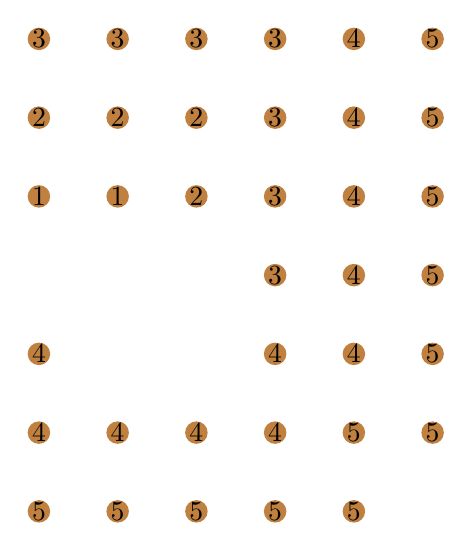
\begin{tikzpicture}[dist/.style={fill=brown, inner sep=0, circle}]\goban{7}{7};\bm{(1, 2)}\bm{(0, 3)}\wm{(1, 3)}\wm{(2, 3)}\bm{(2, 2)}
\node[dist] at (0,0) {\circled{$5$}};
\node[dist] at (1,0) {\circled{$5$}};
\node[dist] at (2,0) {\circled{$5$}};
\node[dist] at (3,0) {\circled{$5$}};
\node[dist] at (4,0) {\circled{$5$}};
\node[dist] at (0,1) {\circled{$4$}};
\node[dist] at (1,1) {\circled{$4$}};
\node[dist] at (2,1) {\circled{$4$}};
\node[dist] at (3,1) {\circled{$4$}};
\node[dist] at (4,1) {\circled{$5$}};
\node[dist] at (5,1) {\circled{$5$}};
\node[dist] at (0,2) {\circled{$4$}};
\node[dist, fill=none, white] at (1,2) {\circled{$3$}};
\node[dist, fill=none, white] at (2,2) {\circled{$3$}};
\node[dist] at (3,2) {\circled{$4$}};
\node[dist] at (4,2) {\circled{$4$}};
\node[dist] at (5,2) {\circled{$5$}};
\node[dist] at (3,3) {\circled{$3$}};
\node[dist] at (4,3) {\circled{$4$}};
\node[dist] at (5,3) {\circled{$5$}};
\node[dist] at (0,4) {\circled{$1$}};
\node[dist] at (1,4) {\circled{$1$}};
\node[dist] at (2,4) {\circled{$2$}};
\node[dist] at (3,4) {\circled{$3$}};
\node[dist] at (4,4) {\circled{$4$}};
\node[dist] at (5,4) {\circled{$5$}};
\node[dist] at (0,5) {\circled{$2$}};
\node[dist] at (1,5) {\circled{$2$}};
\node[dist] at (2,5) {\circled{$2$}};
\node[dist] at (3,5) {\circled{$3$}};
\node[dist] at (4,5) {\circled{$4$}};
\node[dist] at (5,5) {\circled{$5$}};
\node[dist] at (0,6) {\circled{$3$}};
\node[dist] at (1,6) {\circled{$3$}};
\node[dist] at (2,6) {\circled{$3$}};
\node[dist] at (3,6) {\circled{$3$}};
\node[dist] at (4,6) {\circled{$4$}};
\node[dist] at (5,6) {\circled{$5$}};
\markstone[green!90!black]{2}{3}
\end{tikzpicture}
} \end{subfigure}
\begin{subfigure}[b]{.4\textwidth}
\scalebox{.7}{
\begin{tikzpicture}[dist/.style={fill=brown, inner sep=0, circle}]\goban{7}{7};\bm{(1, 2)}\bm{(3, 2)}\wm{(1, 3)}\wm{(2, 3)}\bm{(2, 2)}\bm{(0, 3)}
\node[dist] at (0,1) {\circled{$4$}};
\node[dist] at (1,1) {\circled{$4$}};
\node[dist] at (2,1) {\circled{$4$}};
\node[dist] at (3,1) {\circled{$4$}};
\node[dist] at (4,1) {\circled{$4$}};
\node[dist] at (0,2) {\circled{$4$}};
\node[dist, fill=none, white] at (1,2) {\circled{$3$}};
\node[dist, fill=none, white] at (2,2) {\circled{$3$}};
\node[dist, fill=none, white] at (3,2) {\circled{$3$}};
\node[dist] at (4,2) {\circled{$4$}};
\node[dist] at (3,3) {\circled{$3$}};
\node[dist] at (4,3) {\circled{$4$}};
\node[dist] at (0,4) {\circled{$1$}};
\node[dist] at (1,4) {\circled{$1$}};
\node[dist] at (2,4) {\circled{$2$}};
\node[dist] at (3,4) {\circled{$3$}};
\node[dist] at (4,4) {\circled{$4$}};
\node[dist] at (0,5) {\circled{$2$}};
\node[dist] at (1,5) {\circled{$2$}};
\node[dist] at (2,5) {\circled{$2$}};
\node[dist] at (3,5) {\circled{$3$}};
\node[dist] at (4,5) {\circled{$4$}};
\node[dist] at (0,6) {\circled{$3$}};
\node[dist] at (1,6) {\circled{$3$}};
\node[dist] at (2,6) {\circled{$3$}};
\node[dist] at (3,6) {\circled{$3$}};
\node[dist] at (4,6) {\circled{$4$}};
\begin{scope}\pgfsetfading{fading3}{\pgftransformshift{\pgfpoint{3cm}{2cm}}};\fill [green, even odd rule] (3, 2) circle (.6) circle (.45);\end{scope}\end{tikzpicture}
} \end{subfigure}
\begin{subfigure}[b]{.4\textwidth}
\scalebox{.7}{
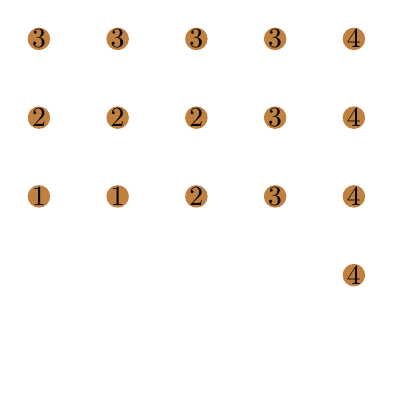
\begin{tikzpicture}[dist/.style={fill=brown, inner sep=0, circle}]\goban{7}{7};\bm{(1, 2)}\bm{(3, 2)}\wm{(1, 3)}\wm{(2, 3)}\wm{(3, 3)}\bm{(2, 2)}\bm{(0, 3)}
\node[dist, fill=none, white] at (1,2) {\circled{$4$}};
\node[dist, fill=none, white] at (2,2) {\circled{$4$}};
\node[dist, fill=none, white] at (3,2) {\circled{$4$}};
\node[dist] at (4,3) {\circled{$4$}};
\node[dist] at (0,4) {\circled{$1$}};
\node[dist] at (1,4) {\circled{$1$}};
\node[dist] at (2,4) {\circled{$2$}};
\node[dist] at (3,4) {\circled{$3$}};
\node[dist] at (4,4) {\circled{$4$}};
\node[dist] at (0,5) {\circled{$2$}};
\node[dist] at (1,5) {\circled{$2$}};
\node[dist] at (2,5) {\circled{$2$}};
\node[dist] at (3,5) {\circled{$3$}};
\node[dist] at (4,5) {\circled{$4$}};
\node[dist] at (0,6) {\circled{$3$}};
\node[dist] at (1,6) {\circled{$3$}};
\node[dist] at (2,6) {\circled{$3$}};
\node[dist] at (3,6) {\circled{$3$}};
\node[dist] at (4,6) {\circled{$4$}};
\markstone[green!90!black]{3}{3}\end{tikzpicture}
} \end{subfigure}
\begin{subfigure}[b]{.4\textwidth}
\scalebox{.7}{
\begin{tikzpicture}[dist/.style={fill=brown, inner sep=0, circle}]\goban{7}{7};\bm{(1, 2)}\bm{(3, 2)}\wm{(1, 3)}\wm{(3, 3)}\wm{(2, 3)}\bm{(4, 3)}\bm{(2, 2)}\bm{(0, 3)}\node[dist, fill=none, white] at (1,2) {\circled{$3$}};
\node[dist, fill=none, white] at (2,2) {\circled{$3$}};
\node[dist, fill=none, white] at (3,2) {\circled{$3$}};
\node[dist, fill=none, white] at (4,3) {\circled{$3$}};
\node[dist] at (0,4) {\circled{$1$}};
\node[dist] at (1,4) {\circled{$1$}};
\node[dist] at (2,4) {\circled{$2$}};
\node[dist] at (3,4) {\circled{$3$}};
\node[dist] at (0,5) {\circled{$2$}};
\node[dist] at (1,5) {\circled{$2$}};
\node[dist] at (2,5) {\circled{$2$}};
\node[dist] at (3,5) {\circled{$3$}};
\node[dist] at (0,6) {\circled{$3$}};
\node[dist] at (1,6) {\circled{$3$}};
\node[dist] at (2,6) {\circled{$3$}};
\node[dist] at (3,6) {\circled{$3$}};
\begin{scope}\pgfsetfading{fading3}{\pgftransformshift{\pgfpoint{4cm}{3cm}}};\fill [green, even odd rule] (4, 3) circle (.6) circle (.45);\end{scope}\end{tikzpicture}
} \end{subfigure}
\captcont{Nombre minimal de pierres noires requises}
\end{figure}

\begin{figure}
\centering
\begin{subfigure}[b]{.4\textwidth}
\scalebox{.7}{
\begin{tikzpicture}[dist/.style={fill=brown, inner sep=0, circle}]\goban{7}{7};\bm{(1, 2)}\bm{(3, 2)}\wm{(1, 3)}\wm{(3, 3)}\wm{(2, 3)}\bm{(4, 3)}\bm{(2, 2)}\bm{(0, 3)}\bm{(3, 4)}
\node[dist, fill=none, white] at (1,2) {\circled{$2$}};
\node[dist, fill=none, white] at (2,2) {\circled{$2$}};
\node[dist, fill=none, white] at (3,2) {\circled{$2$}};
\node[dist, fill=none, white] at (4,3) {\circled{$2$}};
\node[dist] at (0,4) {\circled{$1$}};
\node[dist] at (1,4) {\circled{$1$}};
\node[dist] at (2,4) {\circled{$2$}};
\node[dist, fill=none, white] at (3,4) {\circled{$2$}};
\node[dist] at (0,5) {\circled{$2$}};
\node[dist] at (1,5) {\circled{$2$}};
\node[dist] at (2,5) {\circled{$2$}};
\begin{scope}\pgfsetfading{fading3}{\pgftransformshift{\pgfpoint{3cm}{4cm}}};\fill [green, even odd rule] (3, 4) circle (.6) circle (.45);\end{scope}\end{tikzpicture}
} \end{subfigure}
\begin{subfigure}[b]{.4\textwidth}
\scalebox{.7}{
\begin{tikzpicture}[dist/.style={fill=brown, inner sep=0, circle}]\goban{7}{7};\bm{(1, 2)}\bm{(3, 2)}\wm{(1, 3)}\wm{(3, 3)}\wm{(2, 3)}\bm{(4, 3)}\bm{(2, 2)}\bm{(0, 3)}\bm{(3, 4)}\bm{(2, 5)}
\node[dist, fill=none, white] at (1,2) {\circled{$1$}};
\node[dist, fill=none, white] at (2,2) {\circled{$1$}};
\node[dist, fill=none, white] at (3,2) {\circled{$1$}};
\node[dist, fill=none, white] at (4,3) {\circled{$1$}};
\node[dist] at (0,4) {\circled{$1$}};
\node[dist] at (1,4) {\circled{$1$}};
\node[dist, fill=none, white] at (2,5) {\circled{$1$}};
\node[dist, fill=none, white] at (3,4) {\circled{$1$}};
\begin{scope}\pgfsetfading{fading3}{\pgftransformshift{\pgfpoint{2cm}{5cm}}};\fill [green, even odd rule] (2, 5) circle (.6) circle (.45);\end{scope}\end{tikzpicture}
} \end{subfigure}
\begin{subfigure}[b]{.4\textwidth}
\scalebox{.7}{
\begin{tikzpicture}[dist/.style={fill=brown, inner sep=0, circle}]\goban{7}{7};\bm{(1, 2)}\bm{(3, 2)}\wm{(1, 3)}\wm{(3, 3)}\wm{(2, 4)}\wm{(2, 3)}\bm{(4, 3)}\bm{(2, 2)}\bm{(2, 5)}\bm{(3, 4)}\bm{(0, 3)}
\node[dist, fill=none, white] at (1,2) {\circled{$1$}};
\node[dist, fill=none, white] at (2,2) {\circled{$1$}};
\node[dist, fill=none, white] at (3,2) {\circled{$1$}};
\node[dist, fill=none, white] at (4,3) {\circled{$1$}};
\node[dist] at (0,4) {\circled{$1$}};
\node[dist] at (1,4) {\circled{$1$}};
\node[dist, fill=none, white] at (2,5) {\circled{$1$}};
\node[dist, fill=none, white] at (3,4) {\circled{$1$}};
\markstone[green!90!black]{2}{4}
\markstone[green!90!black]{2}{3}
\end{tikzpicture}
} \end{subfigure}
\begin{subfigure}[b]{.4\textwidth}
\scalebox{.7}{
\begin{tikzpicture}[dist/.style={fill=brown, inner sep=0, circle}]\goban{7}{7};\bm{(1, 2)}\bm{(3, 2)}\wm{(1, 3)}\wm{(3, 3)}\bm{(1, 4)}\wm{(2, 4)}\wm{(2, 3)}\bm{(4, 3)}\bm{(2, 2)}\bm{(2, 5)}\bm{(3, 4)}\bm{(0, 3)}\begin{scope}\pgfsetfading{fading3}{\pgftransformshift{\pgfpoint{1cm}{4cm}}};\fill [green, even odd rule] (1, 4) circle (.6) circle (.45);\end{scope}\end{tikzpicture}}
\end{subfigure}
\caption{Nombre minimal de pierres noires requises}\label{fig:nombre-minimal-pierres}
\end{figure}

On considère le graphe des coups possibles de $\B$. Les sommets du graphe sont les positions possibles, les arcs les coups de $\B$ et le poids des arcs le nombre de pierres noires qu'on ajoute en y jouant. On se rappelle que jouer sur une intersection libre ajoute une pierre noire tandis que jouer sur une pierre noire n'augmente pas le nombre de pierres en jeu. Nous utilisons ensuite l'algorithme de Dijkstra pour calculer le nombre de pierres noires minimales requises pour rejoindre l'origine de toutes les positions. L'utilisation d'une structure de données de type tas (heap en anglais) permet d'obtenir à la ligne \ref{pop} le tuple de distance minimale par l'opération $pop$.

\begin{algorithm}
\fontsize{10}{10}\selectfont
\begin{algorithmic}[1]
\Ensure Le tableau $distances$ correctement mis à jour pour le prochain coup
\Procedure{CalculDesDistances}{}
\State initialisation des distances à $\infty$
\State initialisation du tas $H$
\State marquer $(0,0)$ comme solutionné
\State ajouter $(1, W+(0,1))$ à $H$
\State ajouter $(1, W+(1,1))$ à $H$
\While{$|H| > 0$}
	\State $(d, pt) \gets pop(H)$ \label{pop}
	\If{$pt$ n'est pas solutionné}
		\State $distances[pt] \gets d$
		\ForAll {voisin de $pt$ non-solutionné $v$}
			\If{$v$ est noir}
				\State ajouter $(d, v)$ à $H$
			\ElsIf{$v$ est vide et $d <$ nombre de pierres noires restantes}\label{troploins}
				\State ajouter $(d+1, v)$ à $H$
			\EndIf
		\EndFor
		\State marquer $pt$ comme solutionné
	\EndIf
\EndWhile
\EndProcedure
\end{algorithmic}
\caption{Calcul des distances}\label{algo:calcul-des-distances}
\end{algorithm}


On notera finalement qu'à la ligne \ref{troploins} on évite de traiter une intersection qui se trouve à une distance plus grande que le nombre de pierres noires restantes. Elle demeure, ainsi que toutes les autres intersections qui en dépendent pour leur chemin minimal, hors de portée pour le reste de la partie. La figure \ref{fig:nombre-minimal-pierres} illustre la progression du nombre de positions calculées par l'algorithme tout au long d'une partie.

\subsection{Résultats expérimentaux}

Les résultats expérimentaux présentés ici ont été obtenus en deux temps. Tout d'abord pour \cite{FGLT} nous avons développé l'algorithme principal des gominos. Les temps de calcul étant très long, plusieurs ordinateurs ont été utilisés en parallèle. Les résultats pour les polyominos de périmètre de site jusqu'à $n=15$ ont ainsi été obtenus tels que rapportés au tableau \ref{table:Results}.

Suite à une discussion avec Jérôme Fortier, j'ai remplacé les heuristiques de distances utilisées jusque là par l'algorithme de calcul présenté plus haut. On constate l'amélioration massive des performance sur le graphique \ref{table:Results}.

\begin{table}[!h]
\begin{center}
\scriptsize{
\begin{tabular}{!{\thickvline}c!{\thickvline}c|c|c!{\thickvline}}
\thickhline
$n$ & Simplement 4-connexe & Simplement 8-connexe & 8-trous permis \\
\thickhline
4 & 1 &  1 & 1 \\
\hline
5 & 0 & 0  & 0 \\
\hline
6 & 2 & 2  & 2 \\
\hline
7 & 4 & 4 & 4 \\
\hline
8 & 12 & 12  & 12 \\
\hline
9 & 32 & 32  & 32 \\
\hline
10 & 110 &  110 & 110 \\
\hline
11 & 340 &  340 & 340 \\
\hline
12 & 1193 & 1209 & 1209 \\
\hline
13 & 4080 &  4256 & 4272 \\
\hline
14 & 14786 &  15974 & 16166 \\
\hline
15 & 53428 &  60232 & 61849 \\
\thickhline
\end{tabular}}
\caption{Nombre de polyominos de périmètre de site $n$ selon leur connectivité.}
\label{table:Results}
\end{center}
\end{table}


La taille de l'arbre des parties exploré par l'algorithme peut être borné grossièrement par $7^{2n+1}$ puisque $\B$ a accès à au plus 7 coups possibles, et ne peut pas jouer plus de $2n$ coups puisqu'il lui est impossible de se déplacer plus de 2 fois sur une intersection donnée (sinon $\W$ ne pourrait pas le rejoindre). Le nombre total de parties, tout comme le nombre de parties où $\B$ gagne, est donc borné par une courbe exponentielle. Il serait intéressant d'établir des bornes plus serrées.

En fait, il serait intéressant d'analyser plus en détail la relation entre le nombre de parties de gomino avec moins de $n$ pierres noires et le nombres de parties où $\B$ gagne puisque le graphe à la figure \ref{fig:GominoesVStime} suggère une relation polynomiale entre le temps de calcul (autrement dit le nombre de parties examinées) et le nombre de polyominos (simplement $4$-connexe en bleu, simplement $8$-connexe en rouge). Plus précisément, pour un $n$ donné avec $i=0$ si on inclut les trous, $i=1$ sinon, soit $\gamma_i(n)$ le total de parties de gomino de $≤ n$ pierres et $\beta_i(n)$ le nombre de parties où $\B$ gagne. Une régression linéaire sur ces données avec $R^2=0.9985$ suggère qu'on a
\begin{equation}
\gamma_0(n) \approx \beta_0(n)^{2.0376} \quad \mbox{et} \quad \gamma_1(n) \approx \beta_1(n)^{1.6665} \mbox.
\end{equation}

Toutefois, les nouvelles données obtenues à l'aide de l'algorithme \ref{algo:calcul-des-distances} tendent à montrer que la différence observée entre ces deux courbes était surtout due à l'exploration inutile de boucles intérieures. Les courbes marquées de $\times$ sont maintenant très proches l'une de l'autre.

\begin{figure}[h!]
\centering
\begin{tikzpicture}
\begin{loglogaxis}[xlabel=Nombre de gominos,ylabel=Temps (minutes), title=Temps de calculs]
\addplot[color=red,only marks,mark=o] coordinates {
(1,0.0005)
(3,0.001667)
(7,0.0177)
(19,0.0845)
(51,0.918)
(161,6.1)
(501,66.4)
(1710,426.8)
(5966,4110.98)
(21940,24167.9)
(82172,231715)
};
\addplot[red] table[row sep=\\,
y={create col/linear regression={y=Y}}] % compute a linear regression from the input table
{
X Y\\
1 0.0005 \\
3 0.001667 \\
7 0.0177 \\
19 0.0845 \\
51 0.918 \\
161 6.1 \\
501 66.4 \\
1710 426.8 \\
5966 4110.98 \\
21940 24167.9 \\
82172 231715 \\
};
\addplot[color=blue,only marks,mark=o] coordinates {
(1,0.00033)
(3,0.001)
(7,0.007)
(19,0.02567)
(51,0.175667)
(161,0.721167)
(501,4.62977)
(1694,20.351)
(5774,163.442)
(20560,724.368)
(73988,4878.44)
};
\addplot[blue] table[row sep=\\,
y={create col/linear regression={y=Y}}] % compute a linear regression from the input table
{
X Y\\
1 0.00033 \\
3 0.001 \\
7 0.007 \\
19 0.02567 \\
51 0.175667 \\
161 0.721167 \\
501 4.62977 \\
1694 20.351 \\
5774 163.442 \\
20560 724.368 \\
73998 4878.44 \\
};
\addplot[red] table[row sep=\\,
y={create col/linear regression={y=Y}}] % compute a linear regression from the input table
{
X Y\\
1 0.00142114957173667 \\
3 0.00277415116628333 \\
7 0.00913708209991667 \\
19 0.0274146000545000 \\
51 0.0900924166043333 \\
161 0.291623016198333 \\
501 1.03383256594333 \\
1710 3.67738921641667 \\
5966 13.6965750018833 \\
21940 54.9686681866667 \\
};
\addplot[color=red, only marks,mark=x] coordinates {
(1, 0.00142114957173667)
(3, 0.00277415116628333)
(7, 0.00913708209991667)
(19, 0.0274146000545000)
(51, 0.0900924166043333)
(161, 0.291623016198333)
(501, 1.03383256594333)
(1710, 3.67738921641667)
(5966, 13.6965750018833)
(21940, 54.9686681866667)
};
\addplot[blue] table[row sep=\\,
y={create col/linear regression={y=Y}}] % compute a linear regression from the input table
{
X Y\\
1 0.00132958491643 \\
3 0.00295776923498 \\
7 0.0102820674578 \\
19 0.028353369236 \\
51 0.104771582286 \\
161 0.315272331238 \\
501 1.05738173326 \\
1694 3.76224536896 \\
5774 13.8419382175 \\
20560 51.4730338494 \\
73988 200.061696053 \\
};
\addplot[color=blue, only marks,mark=x] coordinates {
(1, 0.00132958491643)
(3, 0.00295776923498)
(7, 0.0102820674578)
(19, 0.028353369236)
(51, 0.104771582286)
(161, 0.315272331238)
(501, 1.05738173326)
(1694, 3.76224536896)
(5774, 13.8419382175)
(20560, 51.4730338494)
(73988, 200.061696053)
};



\end{loglogaxis}
\end{tikzpicture}
\caption{Temps de calcul des deux premières colonnes du tableau \ref{table:Results}. (L'algorithme original est marqué par des $\protect\circ$ tandis que l'algorithme optimisé est marqué par des $\protect\times$)}
\label{fig:GominoesVStime}
\end{figure}



